\chapter{Theoretische Grundlagen}
In diesem Kapitel werden die theoretischen Grundlagen der Zeitreihe und möglicher Analyseformen, genauso wie die Theorie der Referenzmodellierung und die Systematik der Anforderungserhebung und  Produktauswahl erläutert.

\section{Grundlagen der Datenanalyse}\label{chap:GrundlagenDatenanalyse}

Mathematisch ausgedrückt besteht eine Zeitreihe (im englischen auch \enquote{time series} genannt) aus einer endlichen Menge an zeitlich aufsteigend sortierten Messwerten $x_{t_1},x_{t_2},...,x_{t_T};  x_{t_k} \in \mathbb{R}^n, k=1,2,...,T$, wofür $t_1 < t_2 < t_T $ gilt.\footcite[Vgl.][1]{Deistler.2018b} Zeitreihendaten sind in verschiedenen Feldern zu finden, beispielsweise im Bereich der Aktienmärkte, wo die Preise der einzelnen Kurse abgebildet werden, im Bereich der Gesundheitsforschung, wo die Ansteckungsrate ansteckender Krankheiten wie Covid-19 verfolgt wird oder im Bereich der Sozialwissenschaften, in welchen der Verlauf von Geburtsraten über die Zeit analysiert werden soll.\footcite[Vgl.][1]{Shumway.2017b} In \autoref{abb:BeispielZeitreihe} findet sich beispielhaft die Zeitreihe der verimpften Dosen des COVID-19 Impfstoffes im Januar 2021.

\begin{figure}[H]
\centering
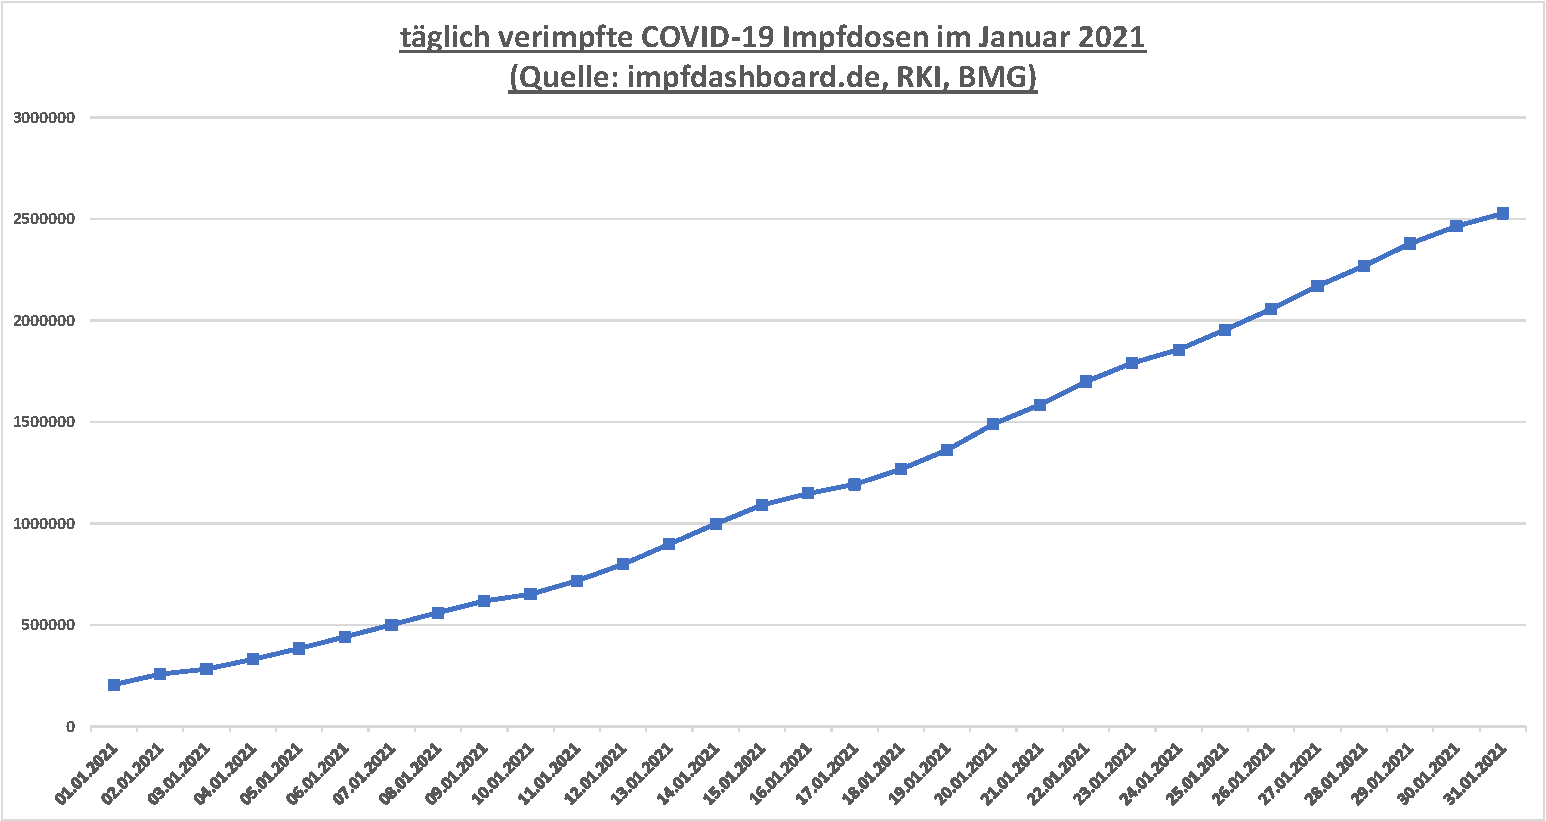
\includegraphics[width=\textwidth]{graphics/Beispiel-Zeitreihe.pdf}
\caption{Beispielhafte Zeitreihe aus dem Januar 2021}
\label{abb:BeispielZeitreihe}
\end{figure}

Die möglichen Anwendungen in der Informatik sind ebenfalls vielzählig. So können über virtuelle oder physikalische Sensoren Messwerte, wie beispielsweise die CPU Auslastung eines gegebenen Servers über die Zeit oder Temperaturmessungen eines \ac{IoT} Gerätes über die Zeit gemacht und gespeichert werden.

Ein wichtiges Merkmal von Zeitreihen ist die Distanz zwischen den Messwerten, im Sinne der Messfrequenz, in welcher Daten betrachtet werden. \Todo{belegen} Ist eine Zeitreihe äquidistant, wurde mit gleichbleibender Frequenz gemessen und die zeitliche Distanz zwischen einzelnen Messwerten ist gleich. Für die in dieser Arbeit diskutierten Auswertungsarten wird eine Äquidistanz der gemessenen Daten angenommen, da andernfalls ein Bias bei der Analyse nicht ausgeschlossen werden kann. Gleichfalls ist es technisch möglich einzelne, nicht äquidistante Messwerte auszusortieren. Die in \autoref{abb:BeispielZeitreihe} abgebildete Zeitreihe ist äquidistant, da die Werte einmal am Tag gesammelt erhoben wurden.


\Todo{Definition Zeitreihendaten}
\Todo{Definition Datenanalyse}

Bei der Verarbeitung von Daten ist zu beachten, dass der Wert, bzw. die Erkentnisse die aus den Daten abgleitet werden können, über die Zeit reduziert wird. \footcite[Vgl. auch im Folgenden][]{NucleusResarchInc..2012} Gemäß \citeauthor{NucleusResarchInc..2012} haben dabei verschiedene Unternehmen verschiedene Zeiträume, in denen Daten nützlich sind, da sie sich in eine von drei Entscheidungstempos einkategorisieren lassen.\footcite[Vgl. auch im Folgenden][3]{NucleusResarchInc..2012} Die Entscheidungstempos sind taktisch, operativ und strategisch. Beim taktischen Entscheidungstempo werden Änderungen sehr schnell, nahe Echtzeit getroffen und implementiert. Im Gegensatz dazu werden Entscheidungen der operativen und strategischen Entscheidungstempi respektive erst in Tagen bzw. Wochen oder innerhalb einem Quartal oder länger implementiert. Je nach Entscheidungstempo sind Analysen von eingehenden Daten also wesentlich früher notwendig oder können beispielsweise auch nur einmal täglich erstellt werden.

% \footcite[Vgl. auch im Folgenden][3]{NucleusResarchInc..2012}
% The value of data diminishes based on the cadence of decisions. Decision tempos are
% tactical (driving process changes in near real time), operational (driving changes that take
% days or weeks to implement), or strategic (driving changes that become part of a quarterly
% or longer planning and implementation process). The concept of half life, with diminishing
% value curves based on a company’s decision tempo, can be used to help companies
% measure the impact of prioritizing their data management and analytics investments. 



Für Unternehmen mit taktischem Entscheidendungstempo haben, gemäß der in \autoref{abb:DataHalflife} gezeigten Befragungsergebnisse von \citeauthor{NucleusResarchInc..2012}, Daten nach maximal 30 Minuten die Hälfte des Wertes eingebüßt.\footcite[Vgl. auch im Folgenden][6]{NucleusResarchInc..2012} Für operative Entscheidungstempi ist die durchschnittliche Halbwertszeit nach acht Stunden erreicht, für strategische Entscheidungstempi nach ca. 56 Stunden, also nach über 2 Tagen.



\begin{figure}[H]
\centering
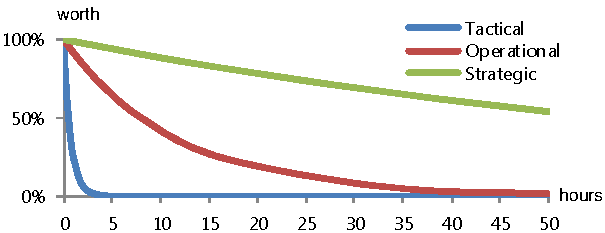
\includegraphics[width=\textwidth]{graphics/half-life-data.pdf}
\caption[Die Halbwertszeit von Daten]{Die Halbwertszeit von Daten\footnotemark}
\label{abb:DataHalflife}
\end{figure}
\footnotetext{Mit Änderungen entnommen aus: \cite{NucleusResarchInc..2012}}
Aus diesen abweichenden Halbwertszeiten und damit aus den abweichenden Zeiträumen, in denen die erhobenen Daten den höchsten Wert haben, ergibt sich die Notwendigkeit von verschiedenen Datenverarbeitungsstrategien, um entsprechend strategischen, taktischen und operativen Entscheidenden die werthaltigsten Daten als Entscheidungsgrundlage zu präsentieren.

\subsection{Arten der Auswertung}
Diese Arbeit soll anhand einiger weniger Auswertungen demonstrieren, wozu die jeweilige Referenzarchitektur und die verwendeten Dienste fähig sind. Im Folgenden werden dazu einige einfachere Auswertungsmethoden für Zeitreihendaten vorgestellt. Die Zeitreihenanalyse und einsetzbare Werkzeuge werden im statistischen Sinn von weiterführenden Werken, wie von \citeauthor{Shumway.2017} behandelt. Es ist davon auszugehen, dass auch weiterführende Auswertungen wie fourieranalytischen Methoden, sofern in der jeweiligen Umgebung bereits vorhanden oder programmierbar, eingesetzt werden können.
\subsubsection{Median}
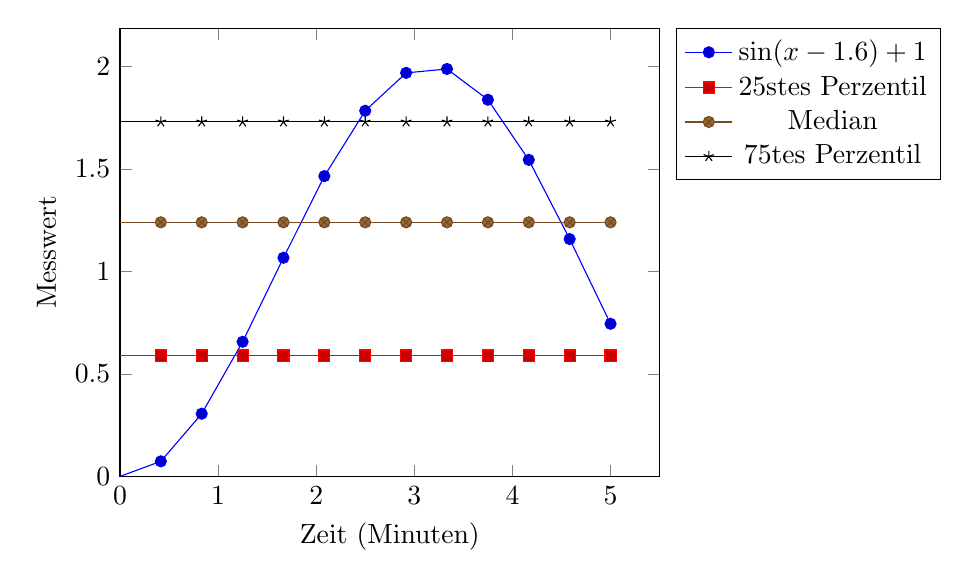
\begin{tikzpicture}
    \begin{axis}[
    xlabel=Zeit (Minuten),
    ylabel=Messwert,
    xmin=0, 
    ymin=0,
    legend pos=outer north east]
        \addplot {sin(deg(x-1.6))+1}; 
        \addplot {0.5899082};
        \addplot {1.2392493};
        \addplot {1.72939505};
        \legend{$\sin(x-1.6)+1$,25stes Perzentil,Median,75tes Perzentil}
    \end{axis}
\end{tikzpicture}


\subsubsection{Anomaliedetektion}
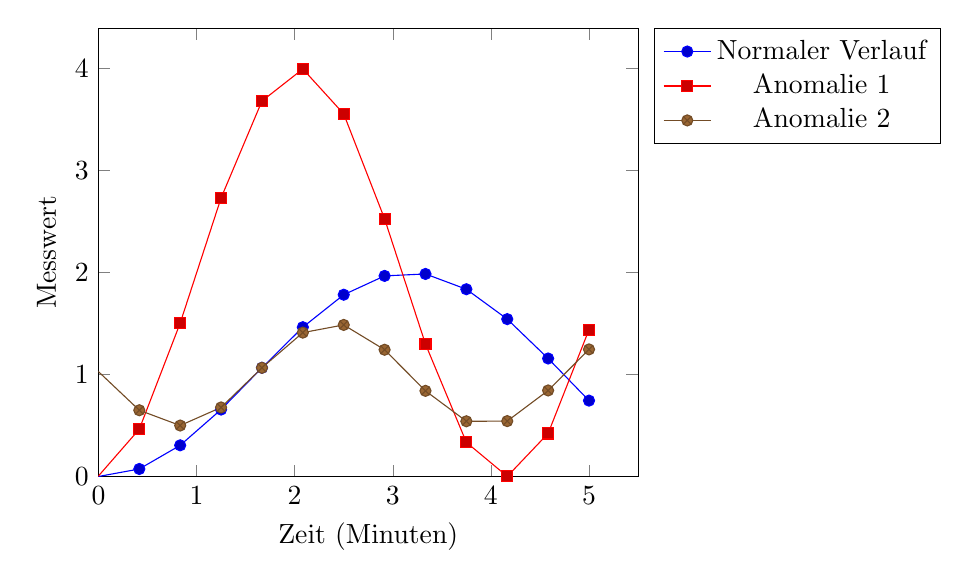
\begin{tikzpicture}
    \begin{axis}[
    xlabel=Zeit (Minuten),
    ylabel=Messwert,
    xmin=0, 
    ymin=0,
    legend pos=outer north east]
        \addplot {sin(deg(x-1.6))+1}; 
        \addplot {2*sin(1.5*deg(x-1))+2};
        \addplot {0.5*sin(2*deg(x-1.6))+1};
        \legend{Normaler Verlauf,Anomalie 1,Anomalie 2}
    \end{axis}
\end{tikzpicture}

\subsubsection{Schwellwertüberschreitung}

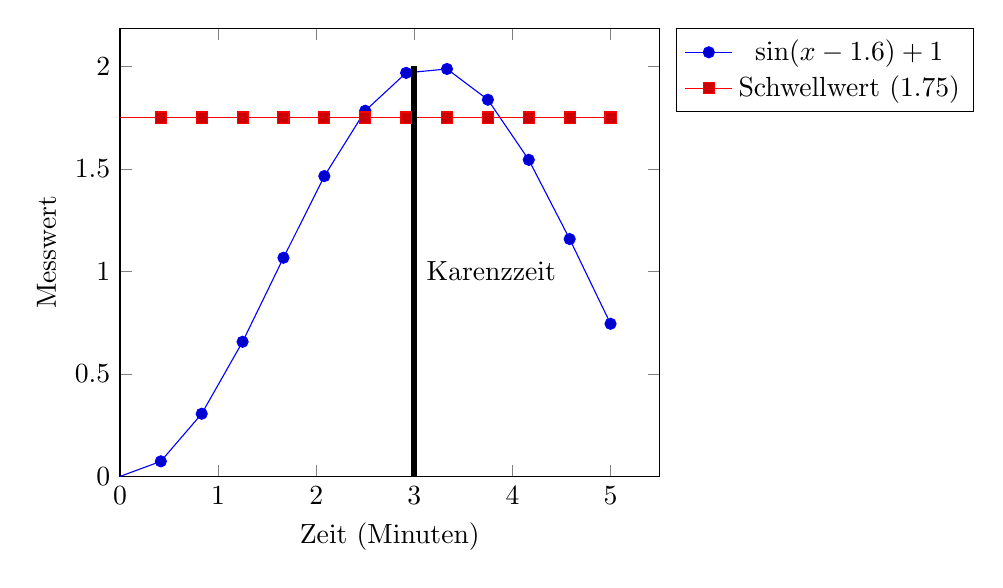
\begin{tikzpicture}
    \begin{axis}[
    xlabel=Zeit (Minuten),
    ylabel=Messwert,
    xmin=0, 
    ymin=0,
    legend pos=outer north east]
        \addplot {sin(deg(x-1.6))+1}; 
        \addplot {1.75};
        \draw [line width=0.8mm, black](axis cs:3,0) -- node[right]{Karenzzeit} (axis cs:3,2);
        \legend{$\sin(x-1.6)+1$,Schwellwert ($1.75$)}
    \end{axis}
\end{tikzpicture}

\subsubsection{Trenderkennung/gleitender Durchschnitt}


% \Todo{Grafik Data Analytics Pipeline}
\begin{figure}[H]
\centering
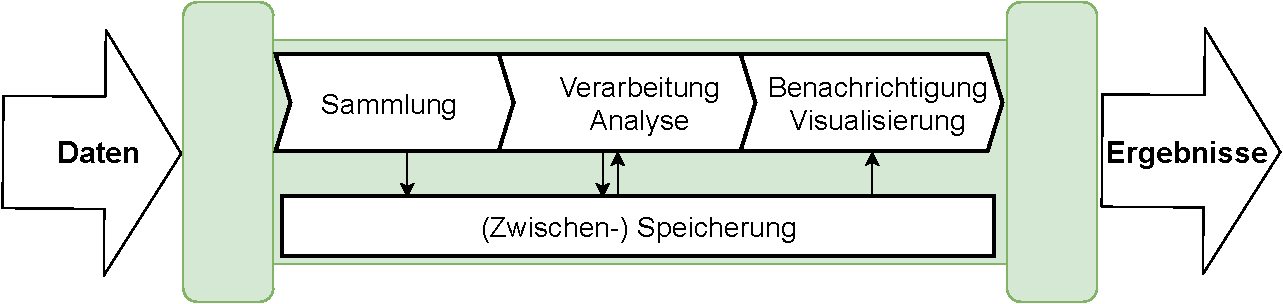
\includegraphics[width=\textwidth]{graphics/DataPipeline.pdf}
\caption{Aufbau und Ablauf in einer Data Pipeline}
\label{abb:DataPipeline}
\end{figure}
\Todo{Quellenangabe}


\subsection{Bestehende Referenzarchitekturkategorien}
Im Bereich der Streamingarchitekturen gibt es bereits etabblierte Referenzarchitekturen, welche verschiedene mögliche Aufbauarten einer Verarbeitung von Streaming/Zeitseriendaten zeigen.

% \Todo{Lambda, Kappa, OLAP elaborieren}
\begin{figure}[H]
\centering
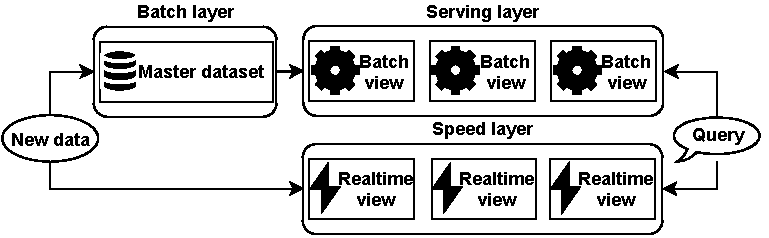
\includegraphics[width=\textwidth]{graphics/Lambda-Reference-Architecture.pdf}
\caption[$\lambda$-Datenstreaming Referenzarchitetktur]{$\lambda$-Datenstreaming Referenzarchitetktur.\footnotemark}
\label{abb:LambdaStreaming}
\end{figure}
\footnotetext{Mit Änderungen entnommen aus: \cite[][28]{Marz.2015}}
% Lambda nach \citeauthor{Marz.2015}, siehe \footcite[Vgl.][28]{Marz.2015}

Die von \citeauthor{Marz.2015} vorgestellte $\lambda$/Lambda-Architektur, welche in \autoref{abb:LambdaStreaming} gezeigt wird ist dabei eine der sehr bekannten Referenzarchitekturen. Der Name ist dabei nicht mit dem \ac{AWS} Dienst Lambda zu verwechseln, sondern ist wohl auf den gedrehten Buchstaben $\lambda$ zurückzuführen, also \reflectbox{\rotatebox[origin=c]{270}{$\lambda$}}.\footcite[Vgl. auch im Folgenden][]{Berle.27.11.2017} Die $\lambda$-Architektur sieht ausgehend von den hereingeladenen Daten zwei verschiedene Wege für die Daten vor. Zum einen den \enquote{Speed Layer}, welcher Daten direkt nach Eingang verarbeitet und nicht im Layer selbst speichert, sondern nur Aggregate oder Ergebnisse zur Verfügung stellt. Zum anderen gibt es den \enquote{Batch layer}, in welchem Daten zuerst in einem Master dataset gespeichert werden und dann in einem festen Intervall (\enquote{Batch jobs}) ausgewertet werden. Verschiedene Datenverarbeitungsintervalle machen speziell im Sinne der verschiedenen, in \autoref{abb:DataHalflife} gezeigten, Datenhalbwertszeiten Sinn. So sind manche Auswertungen, die präzise historische Daten benötigen in einem Batch layer besser möglich als in einem speed layer. Der speed layer bietet dagegen durch die Geschwindigkeit der Auswertungen die möglichkeit, agil auf erkannte Ereignisse oder Veränderungen im generellen zu reagieren.


\begin{figure}[H]
\centering
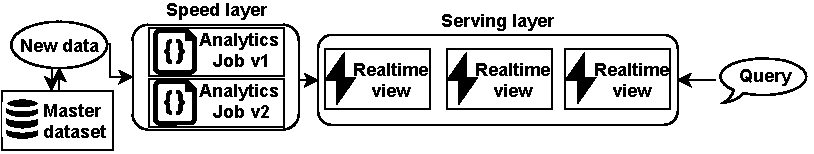
\includegraphics[width=\textwidth]{graphics/Kappa-Reference-Architecture.pdf}
\caption[$\kappa$-Datenstreaming Referenzarchitetktur]{$\kappa$-Datenstreaming Referenzarchitetktur.\footnotemark}
\label{abb:KappaStreaming}
\end{figure}
\footnotetext{Mit Änderungen entnommen aus: \cite{Kreps.2014}, \cite{Berle.27.11.2017}}

Die $\kappa$/Kappa Referenzarchitektur von \citeauthor{Kreps.2014}, dargestellt in \autoref{abb:KappaStreaming} basiert auf der $\lambda$-Architektur, spart jedoch den \enquote{Batch layer} mit zugehörigen \enquote{Batch jobs} aus. Das Konzept von Master Data existiert dabei weiterhin, jedoch in Form von Nachrichten, die in einem Messagebroker gespeichert werden. Analysen werden in Form von einzelnen, unveränderlichen Jobs über die vorhandenen Nachrichten erstellt. Wird die Analyse in irgendeiner Weise verändert (z.B. durtch Codeanpassungen) werden alle zwischengespeicherten Nachrichten erneut durch eine neue, unveränderliche Version des Jobs analysiert. Diese Unveränderlichkeit hat den Vorteil, dass keine unerwünschten Seiteneffekte durch Analysen, die gegenseitig Ergebnisse überschreiben auftreten. \Todo{elaborate on original source}

% Kappa nach \citeauthor{Kreps.2014},
% siehe \footcite[Vgl.][]{Kreps.2014}



\begin{figure}[H]
\centering
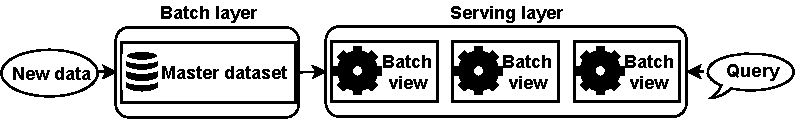
\includegraphics[width=\textwidth]{graphics/OLAP-Reference-Architecture.pdf}
\caption[OLAP Referenzarchitetktur]{OLAP Referenzarchitetktur.\footnotemark}
\label{abb:OLAPStreaming}
\end{figure}
\footnotetext{Mit Änderungen entnommen aus: \cite{Kreps.2014}}

%\ac{OLAP}
Aus der $\lambda$ Referenzarchitektur lässt sich auch eine, zur $\kappa$ Architektur gegenteilige Architektur aufzeigen, welche ein klassisches \ac{OLAP} Szenario aufzeigt. \Todo{Codd zitieren} Diese Architektur basiert, wie in \autoref{abb:OLAPStreaming} gezeigt, auf einer periodischen Verarbeitung der Daten im Master dataset. Dieses Vorgehen ist bei traditionellen Analytics weit verbreitet, bietet jedoch womöglich wichtige Einsichten erst nachdem die Datenhalbwertszeit bereits überschritten wurde.



\subsection{Echtzeitverarbeitung}
Gemäß der in \autoref{abb:KappaStreaming} gezeigten $\kappa$-Architektur gibt es Nutzungsfälle, in welchen eine reine Echtzeitauswertung basierend auf einer Datenquelle, wie beispielsweise dem Messagebroker Sinn machen kann. \citeauthor{Belur.2020} sieht dabei vier verschiedene Verwendungszwecke, in welchen die niedrige Verarbeitungslatenz besonders wichtig ist und den maximalen Wert aus den Daten zieht.\footcite[Vgl. auch im Folgenden][]{Belur.2020} Durch Echtzeit reporting und die Erstellung von Dashboards können aktuelle Daten schnell übersichtlich aufbereitet werden. Mittels erstellter Regeln, die Schwellwertüberschreitungen und Anomalien detektieren, können Nutzende benachrichtigt werden, sobald es zu einer Abweichung kommt. Ebenfalls sinnvoll ist Machine Learning zum auffinden von Mustern in den Daten zu verwenden, was verbesserte Anomalierkennung, Vorraussagen und ähnliche Features ermöglicht. Ein weiterer valider Usecase der $\kappa$-Architektur ist die Transformation von Daten in gewisse Zielformate, um beispielsweise Drittsysteme anzusprechen.
Requirements:
\begin{itemize}
\item Unified experience for data ingestion and edge processing
\item Versatile out-of-the-box connectivity
\item Scalable stream processing with complex transformations
\item Operationalized business rules and ML models
\item Ability to handle unstructured data and schema drift:
\item Reusability of processing logic
\item Governance and lineage
\end{itemize}

% \subsubsection{Streamanalyse}
% \begin{itemize}
% \item AWS Kinesis Data Analytics/Stream
% \item AWS Lambda
% \end{itemize}

\subsection{Datenbankseitige Verarbeitung}
% \subsubsection{Datenbankabfragen}
% \begin{itemize}
% \item Timestream
% \item Redshift
% \item Athena
% \item Elasticsearch
% \end{itemize}

% \subsubsection{Externe Analyse}
% \begin{itemize}
% \item Amazon EMR
% \item Amazon Glue
% \item AWS Lake Formation
% \end{itemize}
Gemäß der in \autoref{abb:OLAPStreaming} gezeigten \ac{OLAP} Architektur, gibt es, wie für die Echtzeitverarbeitung auch nutzende Unternehmen, die ein Entscheidugnstempo mit höherem Horizont haben. Für diese Entscheidungstypen ist dabei wichtig, dass eine Analyse möglichst viele historische Daten umfasst, aber nicht so wichtig, wie zeitnah diese erstellt werden kann. Eine gängige Möglichkeit um effizient alte Daten zu analysieren stellen \ac{OLAP} Datenbanken dar, welche durch spezielle Indexstrukturen und Optimierungen auf komplexe lesende Abfragen bei großen Datenmengen optimiert wurden. \Todo{belegen} Mittels dieser \ac{OLAP} Datenbanken lassen sich dank der jeweiligen Abfragesprachen und -dialekte komplizierte Abfragen realisieren. Bekanntes Beispiel für so eine Abfragesprache wäre \ac{SQL}, welches einige verschiedene Implementierungen (Dialekte) hat, die verwendet werden können. 


NOTIZEN:
Source -> Stream ingestion -> Stream storage -> Stream processing -> Destination

Talkingpoints gegen Streaming onprem:
Difficult to set up, Difficult to achieve high availability,
Error prone and complex to manage,
Tricky to scale, Integration requires development,Expensive to maintain

Amazon Kinesis Data Streams - Daten verfügbar in 70 Milisekunden

Amazon Kinesis Data Analytics

\section{Referenzarchitektur}\label{theorie:referenzmodellierung}
Nach \citeauthor{Bass.2010} ist eine Referenzarchitektur ein spezialisiertes Referenzmodell, wie in \autoref{abb:RelationshipsReferenceModel} gezeigt, welche in Softwarearchitekturen instanziiert werden kann. \footcite[Vgl.][S.~17~f.]{Bass.2010} 

\begin{figure}[H]
\centering
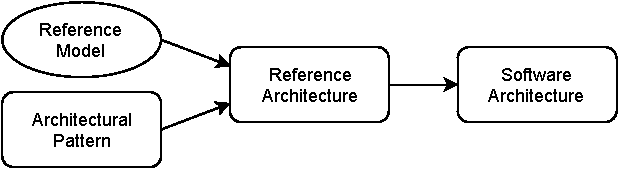
\includegraphics[width=0.66\textwidth]{graphics/Relationships-reference-models.pdf}
\caption[Beziehungen zwischen Referenzmodellen, Architekturpatterns, Referenzarchitekturen und Softwarearchitekturen]{Beziehungen zwischen Referenzmodellen, Architekturpatterns, Referenzarchitekturen und Softwarearchitekturen.\footnotemark}
\label{abb:RelationshipsReferenceModel}
\end{figure}
\footnotetext{Mit Änderungen entnommen aus: \cite[][18]{Bass.2010}}

In diesem Kapitel sollen deshalb die theoretische Definition des Referenzarchitekturbegriffs, genauso wie mögliche Vorgehensmodelle betrachtet werden.



\subsection{Referenzmodelle}

Gemäß des konstruktionsprozessorientierten Referenzmodellbegriffs von \citeauthor{vomBrocke.2003} ist ein Referenzmodell als solches zu erkennen, wenn der Gegenstand und/oder\footnote{Die Verwendung von \enquote{und/oder} wurde hier gewählt, da der Autor der Quelle das \enquote{oder} aus der boolschen Algebra gewählt hat um explizit beide Fälle einzuschliessen.} der Inhalt des Referenzmodells bei der Konstruktion des Gegenstandes und/oder des Inhaltes eines zu konstruierenden Anwendungsmodells wiederverwendet werden kann.\footcite[Vgl.][34]{vomBrocke.2003} Dabei hat ein Referenzmodell einen Empfehlungscharakter und stellt eine \enquote{best practice} dar.\footcite[Vgl.][31]{vomBrocke.2003} 

Ein Referenzmodell kann nach \citeauthor{vomBrocke.2003} nicht objektiv allgemeingültig sein und auch keinen objektiven Empfehlungscharakter haben, sondern muss subjektiv beurteilt werden.\footcite[Vgl. auch im Folgenden][31~f.]{vomBrocke.2003}  Dabei ist zumindest von den Interessensgruppen der Konstruierenden und der Nutzenden auszugehen, welche das Referenzmodell subjektiv unterschiedlich nach Allgemeingültigkeit und Empfehlungscharakter bewerten. Je nachdem welche Beurteilung höher gewichtet wird und früher einfließt, kann also entweder von der Situation ausgegangen werden, dass das Referenzmodell vom Konstruierenden zu einem solchen erklärt wird oder ein Modell, ob vom Konstruierenden beabsichtigt oder nicht, von den Nutzenden zu einem solchen erhoben wird.


\subsection{Referenzarchitektur}
Der IEEE Standard 1471-2000 definiert Architektur im Kontext von softwareintensiven Systemen wie folgt:
\enquote{The fundamental organization of a system embodied in its components, their relationships
to each other, and to the environment, and the principles guiding its design and evolution.} \footcite[][3]{IEEEComputerSociety.2000}. Als softwareintensives System kann jedes System gesehen werden, bei dem Software essentielle Einflüsse auf das Design, die Erstellung, das Deployment oder die Evolution des Systems hat.\footcite[Vgl.][1]{IEEEComputerSociety.2000}

Wird dieser Architekturbegriff auf bekannte Bereitstellungsmodi aus der Cloud, wie \ac{SaaS}, \ac{PaaS}, \ac{IaaS} oder \ac{FaaS} angewendet, wird klar, dass von einer Architektur im Sinne des IEEE Standards 1471-2000 ausgegangen werden kann, sobald Software involviert ist. Im Rahmen dieser Arbeit werden auch Dienste, die sich nach der NIST Cloud Definition unter \ac{SaaS} Dienste zählen lassen, behandelt. Als \ac{SaaS} Dienst gilt dabei jeder Dienst, bei dem Nutzende die unterliegende Infrastruktur nicht verwalten und die Applikation nur über limitierte Konfigurationen verwalten können. Sollte aber die Konfiguration mittels einer Programmiersprache bzw. Datenabfragesprache wie \ac{SQL} erfolgen, ist die Bedingung erfüllt, dass Software wesentliche Einflüsse auf das System hat.


\citeauthor{Gallagher.2000} definiert eine Referenzarchitektur als eine generalisierte Architektur mehrerer Endsysteme, die eine oder mehrere Domänen teilen.\footcite[Vgl. auch im Folgenden][3]{Gallagher.2000} Die Referenzarchitektur definiert nach Sicht des Autors dabei die gemeinsame Infrastruktur der Endsysteme und die Schnitstellen der Komponenten, die in den Endsystemen enthalten sein sollen. Dabei ist eine Referenzarchitektur zu instanziieren, um eine spezifische Softwarearchitektur zu erstellen. Gallagher definiert die Aufgaben einer Referenzarchitektur wie folgt: Zum einen werden übergreifende Funktionen und Konfigurationen generalisiert und extrahiert und zum anderen wird eine kosteneffiziente und verlässliche Basis geschaffen, um Zielsysteme abzuleiten/zu instanziieren.\footcite[Vgl.][3]{Gallagher.2000}

\citeauthor{Trefke.2012} schränkt in seiner Definition die Instanziierung insoweit ein, dass individuelle Besonderheiten abstrahiert werden müssen, um eine Allgemeingültigkeit der Referenzarchitektur in einer speziellen Domäne zu erhalten.  \footcite[Vgl. auch im Folgenden][]{Trefke.2012} Zusätzlich fügt \citeauthor{Trefke.2012} der Referenzarchitektur als optionale Aufgaben die Definition von Leitlinien für die Verwendung, Evolution und Verantwortlichkeiten hinzu. Zurückgreifend auf \citeauthor{vomBrocke.2003} legt \citeauthor{Trefke.2012} fest, dass eine Referenzarchitektur als spezifischeres Referenzmodell seinen Empfehlungscharakter entweder durch Erfahrungen und hohe Nutzerakzeptanz oder durch Festsetzung von Erschaffenden erhält.

Nach \citeauthor{Angelov.2012} gibt es zwei Typen und damit verbundene Zielsetzungen der Referenzarchitektur: Die standardisierende Referenzarchitektur, welche darauf zielt eine Standardarchitektur für spezielle Anwendungsfälle zu schaffen und die unterstützende/erleichternde Referenzarchitektur, welche Personen in Architekturrollen unterstützen sollen, ähnliche Probleme leichter zu lösen.\footcite[Vgl. auch im Folgenden][S.~422~ff.]{Angelov.2012} Nach \citeauthor{Angelov.2012} sind standardisierende Referenzarchitekturen nicht zur Verwendung von innovativen, also kaum getesteten oder noch nicht von Experten akzeptierten Elementen geeignet. Die unterstützenden/erleichternden Referenzarchitekturen hingegen können solche innovativen Elemente durchaus verwenden und auch eine Technologievorauswahl treffen.

Um einen möglichst hohen Nutzen stiften zu können, müssen die organisatorischen Rahmenbedingungen, in welchen ein Referenzmodell eingesetzt werden soll, analysiert werden.\footcite[Vgl.][]{vomBrocke.2004}

%\Todo{What are inputs of a Reference Architecture? - Muller.2020}
\citeauthor{Muller.2020} empfiehlt, eine Referenzarchitektur zur Generalisierung von vorhandenen Architekturen zu verwenden.\footcite[Vgl. auch im Folgenden][7]{Muller.2020} Für neue Technologien und Applikationen, die bislang in der Form kaum verwendet wurden, schlägt \citeauthor{Muller.2020} stattdessen ein inkrementelles Vorgehen vor. Das inkrementelle Vorgehen von \citeauthor{Muller.2020} beinhaltet dabei die Erstellung von Prototypen und Einholung von Feedback der Zielstakeholder. 


\subsection{Diskussion der Qualitätskriterien der Referenzarchitekturen}\label{chap:qualitycriteria}
\citeauthor{Muller.2020} schlägt sieben Qualitätskriterien vor, welche von einer guten Referenzarchitektur erfüllt werden sollten:\footcite[Vgl. auch im Folgenden][8]{Muller.2020}
\begin{enumerate}
\item Verständlichkeit für eine breite, heterogene Gruppe an Stakeholdern (Kunden, Projektmanager, Entwickler, etc.)
\item Zugänglichkeit und Zugriff durch die Mehrheit der Organisation
\item Adressierung der Hauptprobleme der spezifischen Problemdomäne
\item Zufriedenstellende Qualität
\item akzeptabel
\item \enquote{up-to-date} und wartbar
\item wertschöpfend für den Betrieb
\end{enumerate}

\ac{AWS} definiert im Rahmen des sogenannten Well Architected Frameworks für verschiedene \enquote{Lenses}, also Spezialisierungen, Themenfelder, die bei exzellenten Architekturen zu beachten sind. Für Datenanalysen gibt es die Analytics Lens, welche entsprechend für Referenzarchitekturen genauso Anwendung finden sollte. Kriterien sind dabei die Folgenden:\footcite[Vgl.][6]{Ravirala.2020}:
\begin{enumerate}
\item Automate data ingestion
\item Design ingestion for failures and duplicates => Siehe Robustness and fault tolerance
\item Preserve original source data
\item Describe data with metadata
\item Establish data lineage
\item Use the right ETL tool for the job
\item Orchestrate ETL workflows
\item Tier storage appropriately
\item Secure, protect, and manage your entire analytics pipeline
\item Design for scalable and reliable analytics pipelines => Scalability, robustness and fault tolerance
\end{enumerate}


\subsection{Vorgehensmodell}

\citeauthor{Schutte.1998} unterteilt Referenzmodellierung generell in vier Phasen.\footcite[Vgl. auch im Folgenden][184\psq]{Schutte.1998} Die erste Phase, die Problemdefinition ist mit der Darstellung des behandelten Problems in der Einleitung dieser Arbeit bereits vorgenommen worden. Laut \citeauthor{Schutte.1998} kann der Wirklichkeitszugang des erstellten Modells nur über Bilder erfolgen, welche entsprechend zu modellieren sind.\footcite[Vgl. auch im Folgenden][185\psq]{Schutte.1998} Da momentan keine Erfahrungen in den zu verwendenden Technologien für die Referenzmodellierung vorliegt, handelt es sich um eine Top-down Referenzmodellierung/Referenzarchitektur. Bei der Konstruktion des Referenzmodellrahmens wird durch das \enquote{Was} motiviert, welche Unternehmensspezifika zu beachten sind.\footcite[Vgl. auch im Folgenden][186]{Schutte.1998} In der vorliegenden Arbeit wäre beispielsweise Teil des Referenzmodellrahmens, dass cloudbasiert gearbeitet werden soll und dass die Zeitreihendaten vorerst vornehmlich von \ac{IoT} Anwendungsfällen stammen, was sich später dennoch ändern könnte.\footcite[Vgl. auch im Folgenden][187\psq]{Schutte.1998} In der \enquote{Wie} Phase, die dieses Kapitel behandeln soll, wird die Referenzarchitektur strukturiert und Darstellungsarten gezeigt, welche folgend angewendet werden können. 

\begin{figure}[H]
\centering
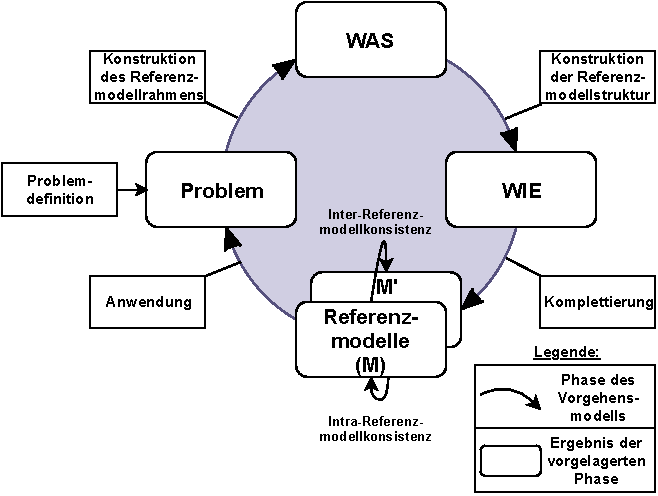
\includegraphics[width=0.75\textwidth]{graphics/Vorgehen-Referenzmodellierung.pdf}
\caption[Vorgehensmodell Referenzmodellierung nach Schütte]{Vorgehensmodell Referenzmodellierung nach Schütte.\footnotemark}
\label{abb:VorgehensmodellReferenzmodellierung}
\end{figure}
\footnotetext{Mit Änderungen entnommen aus: \cite[][185]{Schutte.1998}}




Nach \citeauthor{Muller.2020} hat eine Referenzarchitektur mehrere Dekompositionen, in beispielsweise eine funktionale, eine konstruktionsorientierte oder eine infrastrukturorientierte Komposition.\footcite[Vgl.][7]{Muller.2020} Diese Dekompositionsschichten lassen sich ebenfalls in bekannten Architekturframeworks wie arc42 finden, weshalb diese mit Anpassungen zur Visualisierung dienen sollen. Dies deckt sich auch mit der Auffassung von \citeauthor{Schutte.1998} zur Referenzmodellierung, welcher Modellierung über Bilder erfolgen lassen möchte.\footcite[Vgl.][185]{Schutte.1998}

\begin{figure}[H]
\centering
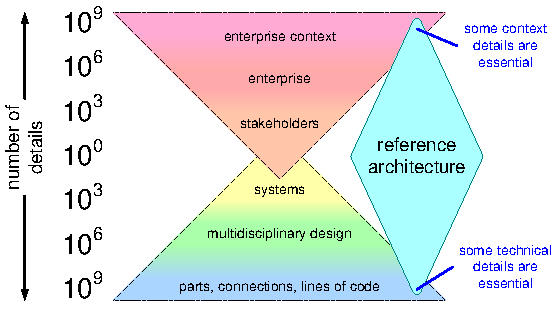
\includegraphics[height=0.23\textheight]{graphics/reference-architecture-details.pdf}
\caption[Gewünschter Detailgrad von Referenzarchitekturen nach \citeauthor{Muller.2020}]{Gewünschter Detailgrad von Referenzarchitekturen nach \citeauthor{Muller.2020}.\footnotemark}
\label{abb:DetailgradMuller}
\end{figure}
\footnotetext{Entnommen aus: \cite[][11]{Muller.2020}}

Mehrere Dekompositionen machen insbesondere auch Sinn, da wie im Diagramm von \citeauthor{Muller.2020} - \autoref{abb:DetailgradMuller} - eine Addressierung von unterschiedlichen Aspekten wie Systemgestaltung, aber auch Stakeholder oder Kontext erfolgen sollte. Eine Adressierung der Stakeholder und des Kontextes ist insofern gegeben, dass, wie in \autoref{chap:requirements} gezeigt, Interviews durchgeführt und im Anhang dieser Arbeit transkribiert werden. An Stellen, an denen ein Einsatz von Teilen der Referenzarchitektur nontrivial scheint, kann durch Codebeispiele oder konkrete, kopierbare \enquote{Schnipsel} gezeigt werden, auf was speziell im technischen Bereich zu achten ist.

Zusätzlich sollen Dekompositionen unterschiedliche Aufgaben erfüllen. Speziell für die Darstellung der verwendeten Diensten von \ac{AWS} in den Referenzarchitekturen und dem Datenfluss soll die erste Stufe der Bausteinsicht des Architekturstandards arc42 verwendet werden. Das Konzept jener Bausteinsicht, also wie sie zu gestalten ist, findet sich in \autoref{abb:BausteinsichtStufe1}. In der finalen Umsetzung werden die offiziellen \ac{AWS} Icons die entsprechenden Services darstellen, die verwendet werden.

\begin{figure}[H]
\centering
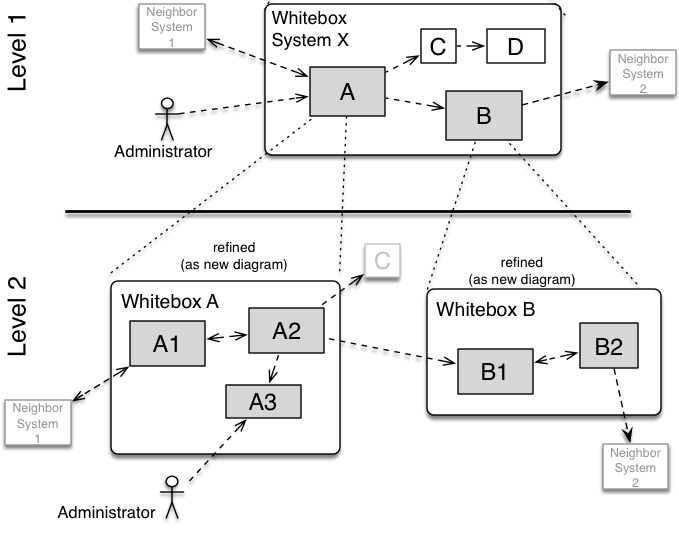
\includegraphics[height=0.38\textheight]{graphics/Bausteinsicht.png}
\caption[Stufe 1 der Bausteinsicht in arc42]{Stufe 1 der Bausteinsicht in arc42.\footnotemark}
\label{abb:BausteinsichtStufe1}
\end{figure}
\footnotetext{Mit Änderungen entnommen aus: \cite{Starke.o.J.}}

Zusätzlich zu der Bausteinsicht können, wie in \autoref{abb:Diagrammtypen} geizeigt, weitere Diagrammtypen eingesetzt werden, um verschiedene Dekompositionen darstellen zu können.

\begin{figure}[H]
\centering
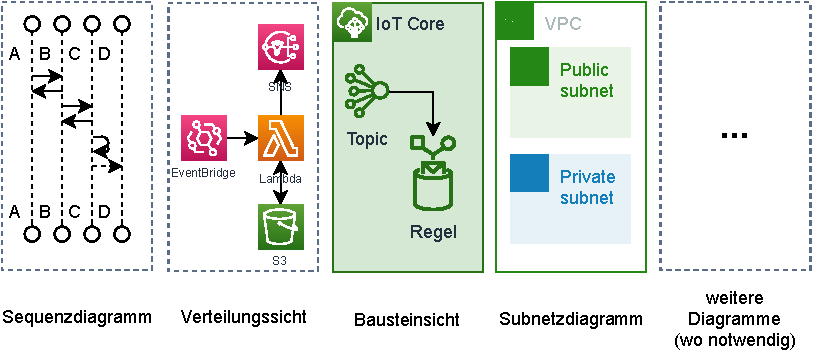
\includegraphics[width=\textwidth]{graphics/Diagrammtypen.pdf}
\caption{Ergänzende Dekompositionen}
\label{abb:Diagrammtypen}
\end{figure}


Wie von \citeauthor{Muller.2020} vorgeschlagen und im vorherigen Unterkapitel erläutert, ist ein inkrementeller Ansatz unter Verwendung von Prototypen und kontinuierlichem Feedback der Zielstakeholder unerlässlich.\footcite[Vgl.][7]{Muller.2020} 

Sehr wichtig für eine Referenzarchitektur ist auch die Dokumentation, wie die Wiederverwendung zu handhaben ist. Ein möglicher Ansatz wäre dabei die gezielte Integration und Dokumentation von Variationspunkten, wie von \citeauthor{Webber.2001} vorgeschlagen.\footcite[Vgl.][24\psqq]{Webber.2001} Mittels der Variationspunkte kann eine statische Referenzarchitektur konstruiert werden, welche an spezifisch definierten Punkten angepasst werden muss, um einzigartige Architekturen zu erzeugen.\footcite[Vgl.][24]{Webber.2001} Dabei gibt es vier verschiedene Ansichten, aus denen Variationspunkte definiert werden können:\footcite[Vgl.][25\psq]{Webber.2001}
\begin{enumerate}
\item \label{view:first} Requirement-Variation-Point View
\item \label{view:second} Component-Variation-Point View
\item \label{view:third} Static-Variation-Point View
\item \label{view:fourth} Dynamic-Variation-Point View
\end{enumerate}
Dabei sind für diese Arbeit, in der keine implementierungsnahe (im Sinne von Programmierung) Softwarearchitektur entworfen wird, hauptsächlich die anforderungsbasierte und die komponentenbasierte Variationspunktsicht aus \autoref{view:first} und \autoref{view:second} wichtig. Die statische und dynamische Variationspunktsicht aus \autoref{view:third} und \autoref{view:fourth} agieren stärker auf Implementierungsebene.\footcite[Vgl. auch im Folgenden][25\psq]{Webber.2001} Auf dieser können beispielsweise mittels objektorientierter Programmierung Klassen bereitgestellt werden, von welchen geerbt werden kann. Gleichzeitig kann die Verhaltensweise des Programms auch durch z.B. Callbacks oder Parameterisierung des Aufrufes verändert werden.

\renewcommand\#{\protect\scalebox{0.8}{\protect\raisebox{0.4ex}{\char"0023}}}

Variationspunkte können, wie in \autoref{abb:Variationspunkte} dargestellt innerhalb der verschiedenen, dargestellten Schichten wie folgt dargestellt werden:
\begin{figure}[H]
\centering

\includegraphics[height=1.33cm]{graphics/Variationpoints.pdf}
\caption{Darstellung Variationspunkte}
\label{abb:Variationspunkte}
\end{figure}
In den Architekturebenen werden entsprechend die Variationspunkte mit durchgängigen Nummern versehen, welche entsprechend vor dem \# stehen.





% Überleitung => generelle Referenzmodelle 
% => Empfehlungscharakter 
% => Anwendung Architektur 
% => Unterlegung Arc42 als Modellierungssprache



\section{Theorie der Anforderungserhebung}\label{chap:requirements}

Gemäß der in \autoref{chap:qualitycriteria} definierten Qualitätskriterien und der von \citeauthor{vomBrocke.2003} aufgestellten Allgemeingültigkeitskriterien kann ein Referenzmodell und damit auch eine Referenzarchitektur nicht objektiv allgemeingültig sein. Zusätzlich ergeben sich als weitere wichtige Eingaben zur Konstruktion eines Referenzmodells die Dekompositionstiefe und die Anwendbarkeit. Zusammen lassen sich diese Dimensionen als Kiviat Diagramm,\footcite[Vgl.][33\psqq]{Kolence.1973} wie in \autoref{abb:Dimensionen} gezeigt, abbilden. Die Dekompositionstiefe misst die Anzahl an Schichten und die Detailtiefe der verschiedenen Dekompositionsschichten die im Rahmen der Architektur verwendet werden. Ein niedriger Wert entspricht einer geringen Anzahl, welche keine große Detailtiefe aufweisen. In \autoref{abb:Diagrammtypen} sind mögliche Dekompositionen mit unterschiedlicher Tiefe gezeigt. Die Anwendbarkeit, als Gegensatz zur Abstraktion misst, wie gut und schnell sich eine Referenzarchitektur instanziieren lässt, um eine spezifische Architektur abzuleiten. Ein niedriger Wert bedeutet eine sehr abstrakte Referenzarchietktur, deren Instanziierung mit viel Aufwand verbunden ist. Die Allgemeingültigkeit beschreibt die Menge an Anwendungsfällen und die Losgelöstheit von Firmenspezifika beziehungsweise die übergreifende Gültigkeit in mehreren Teams. Idealerweise ist eine Referenzarchitektur spezifisch für eine Zielorganisation, aber nicht zu spezifisch, sondern erlaubt Anwendungen in anderen Teams.

\begin{figure}[H]
\centering
\scalebox{0.75}{
    \spider{0}{0}{0}
}

\caption{Referenzarchitekturdimensionen}
\label{abb:Dimensionen}
\end{figure}

Ziel einer Referenzarchitektur sollte also sein, das optimale Verhältnis der drei Dimensionen für die Zielstakeholder zu finden und daraus eine Referenzarchitektur zu erstellen. Um dieses Ziel zu erreichen, sind Interviews mit Zielstakeholdern der SPIRIT/21 zu führen, welche dem Interviewleitfaden in \autoref{tab:intervieleitfaden} folgen. Im referenzierten Leitfaden stehen dabei Fragen mit einem F-Präfix für allgemeine Fragen und Fragen mit einem D-Präfix für Fragen in Bezug auf die drei Dimensionen. Kombiniert mit mindestens einem Review der Referenzmodelle werden die Modelle zu einem nutzenstiftenden Artefakt.



\begin{table}[H]
\centering
\begin{tabular}{|l|l|}
\hline
ID & Beschreibung \\ \hline
\multicolumn{2}{|c|}{\cellcolor[HTML]{ECF4FF}Allgemeine Fragen} \\ \hline
F1 & Rolle innerhalb der SPIRIT/21 \\ \hline
F2 & Anwendungsgebiete der Referenzarchitekturen \\ \hline
F3 & Kompatibilität der Referenzarchitekturen zueinander? \\ \hline
\multicolumn{2}{|c|}{\cellcolor[HTML]{ECF4FF}Priorisierungen} \\ \hline
P1 & Priorisierung der Qualitätskriterien (siehe \autoref{chap:qualitycriteria}) \\ \hline
P2 & Priorisierung der Datennutzungstypen (siehe \autoref{chap:GrundlagenDatenanalyse}) \\ \hline
\multicolumn{2}{|c|}{\cellcolor[HTML]{ECF4FF}Dimensionen der Referenzarchitekturen} \\ \hline
D1 & Anforderungen an Anwendung der Referenzarchitekturen \\ \hline
D2 & Anforderungen an Allgemeingültigkeit der Referenzarchitekturen \\ \hline
D3 & Dekompositionstiefe der Referenzarchitekturen \\ \hline
\end{tabular}
\caption{Interviewleitfaden für Schlüsselstakeholder}
\label{tab:intervieleitfaden}
\end{table}




\section{Vergleichsmethodik für die Produktauswahl}\label{chap:vergleichsmethodik}

\citeauthor{Marz.2015}, die bereits die $\lambda$-Architektur geprägt haben, haben folgende,erwünschte Eigenschaften eines Big Data Systems festegelegt:\footcite[Vgl.][7\psqq]{Marz.2015}
\begin{enumerate}
\item Robustness and fault tolerance

Systeme sollen Herausforderungen, wie beispielsweise Paralellität, Datenduplikate oder technische Ausfälle verkraften. Zusätzlich ist Resilienz gegenüber menschlichen Fehlern wünschenswert, so dass händische Änderungen rückgängig gemacht werden können (also beispielsweise Analysecode \enquote{immutable} ist).
\item Low latency reads and updates

Lesezugriffe auf Daten sollen mit niedriger Latenz stattfinden. Wie bereits beschrieben, kann aufgrund der Messdistanz eine Aktualisierung von Daten durchaus längere Zeit benötigen, jedoch sollte ein Big Data System in der Lage sein, Datenaktualisierungen mit niedriger Latenz durchzuführen.
\item Scalability

Das Big Data System sollte durch transparente oder intransparente Provisionierung weiterer Ressourcen in der Lage sein, gleiche Performance in verschiedenen Belastungssituationen zu liefern. Dies deckt sich mit einem der Kernversprechen der Public Clouds nach NIST Definition (\enquote{rapid elasticity}).\footcite[Vgl.][2]{Mell.2011}
\item Generalization

Ein Big Data System sollte in der Lage sein, verschiedene Anwendungen zu unterstützen. Da die Zielsetzung dieser Bachelorarbeit auf Zeitreihendaten aufbaut, welche wie in \autoref{chap:GrundlagenDatenanalyse} gezeigt, einen großen Einsatzspielraum haben, ist diese Bedingung bei ausreichender Generalisierung der Referenzarchitekturen erfüllt.
\item Extensibility

Das zu gestaltende Big Data System soll erweiterbar sein und neue Funktionen oder Änderungen ohne größeren Aufwand ermöglichen.
\item Ad hoc queries

Diverseste Abfragen sollen schnellstmöglich auf dem Datensatz der Big Data Anwendung möglich sein.
\item Minimal maintenance

Eine Big data Anwendung soll wartbar bleiben, indem Komplexität in den Kernkomponenten, welche nach Ansicht von \citeauthor{Marz.2015} zu erhöhtem Wartungsaufwand führt, möglichst gering ist.
\item Debuggability

Innerhalb eines Big Data Systems soll es möglich sein, nachzuverfolgen, wie Werte entstanden sind, um mögliche Fehler verfolgen zu können.
\end{enumerate}

% Kriterien von Lukas an ein Produkt:
% \begin{itemize}
% \item zufriedenstellende Integration mit AWS nativen Diensten (z.B. Monitoring)
% \item Möglichst serverless (wenig Maintenance Aufwand)
% \item skalierbarkeit auf 0 bis 10000
% \end{itemize}

% Anforderungen von Kunden
% \begin{itemize}
% \item Skalierbarkeit
% \item pay for what you use (no dead infra)
% \item transparente Fehler
% \end{itemize}

% \begin{itemize}
%     \item Übertragbarkeit (ggf. zwischen Clouds)
% \end{itemize}

Vielleicht noch:
Requirements:\footcite[Vgl.][]{Belur.2020}
\begin{itemize}
\item Unified experience for data ingestion and edge processing
\item Versatile out-of-the-box connectivity
\item Scalable stream processing with complex transformations
\item Operationalized business rules and ML models
\item Ability to handle unstructured data and schema drift:
\item Reusability of processing logic
\item Governance and lineage
\end{itemize}

\subsection{Featurevergleich}
Es soll auf die Mindestverfügbarkeit folgender Fähigkeiten überprüft werden:
\begin{itemize}
\item Auswertungen nach \autoref{chap:auswertungsarten}
\end{itemize}

\subsection{Performancevergleich}
Es muss mindestens die theoretische Verarbeitungslatenz verglichen werden

\subsection{Kostenvergleich}
Um einen sinnvollen Kostenvergleich aufzustellen, sind folgende Annahmen zu treffen:
Es existieren 200 Geräte/Sensoren. Es geht eine Nachricht mit einem kB pro Minute pro Gerät ein (0,0432 GB/Gerät/Monat und 8,64 GB/Monat).
Es ist eine Vergleichsoperation auf einen Schwellwert auszuführen und wo möglich eine Zählung aller Schwellwertüberschreitungen der letzten drei Monate durchzuführen (historische Daten also mindestens 25,92 GB).  Es ist die Region Frankfurt (eu-central-1) mit Abrechnungswährung US-Dollar (Umrechnung in € erfolgt bei \ac{AWS} bei Abrechnung) zu wählen alternativ ist die Region Irland (eu-west-1) bei Nichtverfügbarkeit der Diensleistung in Frankfurt zu wählen. Produkte, die diese Analyse alleine nicht bewerkstelligen können, müssen unter zusätzlicher Verwendung von Rechendiensten wie Lambda oder \ac{EC2} angesetzt werden mit permanentem Speicher, der historische Daten speichert (\ac{S3}). Analysen, wo individuell auslösbar erfolgen alle 10 Minuten an Werktagen zwischen 9 und 17 Uhr, also monatlich 960mal. Andernfalls wird angenommen, dass der Schwellwert 5 mal pro Gerät pro Monat überschritten wird (1000 Überschreitungen).
Für die Zwischenspeicherung in \ac{S3}, wenn benötigt, wird folgendes Datenschema angenommen:

\begin{listing}[H]
\inputminted[frame=lines,breaklines=true]{json}{code/estimates/filtered-estimate.json}
\caption[Beispiel JSON]{Beispiel \ac{JSON}}
\label{listing:json}
\end{listing}
Um Historien über 3 Monate bereitzustellen, sind entsprechend 3000 Einträge nötig, was eine Dateigröße von ~455,32 KB ergibt. Das Berechnungsskript ist im Anhang \ref{anhang:berechnung} abgedruckt.


\begin{table}[H]
\centering
\begin{tabular}{|l|l|l|}
\hline
Dimension & Preis/Einheit           & Summe \\ \hline
Beispiel  & x\$/100.000 Datenpunkte & x\$  \\\hline
\end{tabular}
\caption{Kostenvergleich Schema}
\label{tab:kostenvergleich-schema}
\end{table}
Es sind alle Abrechnungsdimensionen in der in \autoref{tab:kostenvergleich-schema} gezeigten Form zu dokumentieren.


